\documentclass[12pt,twoside]{rif}

\pagestyle{myheadings}
\usepackage[
left=2.54cm,
right=2.54cm,
top=2.54cm,
bottom=2.54cm]
{geometry}
\usepackage{hyperref}
\usepackage{natbib}
\usepackage{subfigure}
\hypersetup{
	urlcolor=blue, 
	colorlinks=true, 
	citecolor=blue
}

\usepackage{lipsum}

\title{\textbf{Dilatación del tiempo gravitacional}}

\author[1]{{\small Carlos Andrés García Suarez}} 
\author[1]{{\small David Brandon Zevallos Garay}}
\author[1]{{\small Luis Fernando Ubillus Benites}}
%\author[3]{Autor3}
\affil[1]{{ \small Facultad de Ciencias Naturales y Matemática, Universidad
		Nacional Federico Villarreal. El Agustino 15003. Lima-Perú.}}
%\affil[2,3]{Afiliacion2}
%\date{\normalsize Recibido: xxxx Aceptado: xxxx Publicado: xxxx\\
%Todos los derechos reservados-SEF \copyright{} 2012}
\date{}

\begin{document}
	\maketitle
	
	\begin{res}
		\begin{center}
		%\textbf{Resumen} \\
			En esta monografia se recopilo informacion historica de la dilatacion gravitatoria del tiempo, los experimentos realizados para comprobarlo y los efectos que este tiene en el mundo real. Se presentara la fisica necesaria para entender estos conceptos y finalmente se explicara como sucede esto en una aproximacion  newtoniano para un campo gravitatorio homogeneo y no homogeneo. Seguira con una aplicacion al GPS donde se resalta lo que sucederia no tener en cuenta estos efectos para ciertos calculos y finalmente se analizara como afecta estos efectos en nuestra percepcion del universo.
		\end{center}
		%\lipsum[2]
		
		\par
		\smallskip
		\clav{dilatacion gravitacional, relatividad , principio de equivalencia, campo homogeneo, campo no homogeneo}
	\end{res}
	\begin{center}
		\title{\textbf{Time gravitational dilation}}
	\end{center}
	
	\begin{abst}
		\begin{center}
			\textbf{Abstract} \\
			In this monograph historical information about gravitational time dilation, the experiments performed to prove it and the effects it has in the real world are compiled. The physics necessary to understand these concepts will be presented and finally it will be explained how this happens in a Newtonian approximation for a homogeneous and non-homogeneous gravitational field. We will continue with an application to GPS where we will highlight what would happen if we do not take into account these effects for certain calculations and finally we will analyze how these effects affect our perception of the universe.
		\end{center}
		%\lipsum[2]
		
		\par 
		\smallskip
		\key{gravitational dilation, relativity, equivalence principle, homogeneous field, non-homogeneous field, homogeneous field}
	\end{abst}

	
	
	\newpage
	
	\tableofcontents
	
	\section{ Introducción} 
	La teoria de la relativida especial (RE) es una de las teorias 'anti intuitivas' del siglo XIX junto con la Mecanica
Cuantica, la RE nos da una comprension del universo a medidas macroscopicas para sistemas inerciales, Esta nos da un nuevo
concepto del Espacio y el tiempo Newtoniano, juntado como un solo ente llamado Espacio-Tiempo. (14)
Esta tenia como limites los marcos inerciales (no acelerado con respecto a otro) en 1907 se dio cuenta de la
incompatibilidad con la gravedad Newtoniana, impresionado por la igualdad inercial y gravitatoria debido al experimento 
como el de Lorand Eotvos (2) y mejorado en 1964 por Robert Dicke (3) se sabe que eran equivalentes ambas definiciones de masa.
En 1907 mas tarde se dio cuenta que: \\

 'un observador en caida libre no siente su propio peso y por lo tanto podria pensar que estuviera en una region del espacio donde no hubiera campo gravitarorio' (4) (copia literal)\\

Con este principio pudo generalizar el concepto de observador inercial y obtener las ecuaciones de campo de Einstein que dan
una descripcion de como el espacio-tiempo le dice al "ente" como moverse y como el "ente" deforma el espacio-tiempo(5)
Se hicieron diversos experimentos para comprobar lo que dice la Relatividad General en los limites Newtonianos, uno de ellos 
es el experiento de  Pound y Rebka (6) y en 1964 el experimento de Pound-Snider (7) del corrimiento al rojo de fotones que
escapan de un potencial gravitatorio.
En la epoca actual una aplicacion conocida es la del GPS que tiene que realizar correciones relativista para conseguir la 
sincronizacion (8) o el corrimiento al rojo de las enanas blancas, estudio llevado a cabo en una tesis con datos recopilados de 
Distintas Bases de datos de enanas blancas (9)
	\section{Marco Teórico}
	\subsection{Teoria de la Relatividad Especial}
	Este es el enfoque moderno que le dio Albert Einsten a la fisica, donde se "olvida" el concepto de tiempo y distancia Absoluto de la Teoria de Newton.
	Esta teoria se basa en dos postulados simplemente:
	Las leyes de la Fisica son validas para todos los sistemas "inerciales"
	 La velocidad de la luz en el vacio es igual para todos los observadores 
	Hay que tener cuidado con la palabra inercial que es su campo de aplicacion.
	\subsection{Principio de equivalencia}
	Un punto clave en este trabajo es el principio de equivalencia, que nos dice que un observador en caida libre en un campo gravitatorio es equivalente a un observador en el espacio fuera de toda influencia gravitatoria. Todo esto de forma local hasta que este sienta las consecuencias de la curvatura. Pero tambien nos dicen que un observador acelerado con aceleracion a en el espacio sin influencia de gravedad,es equivalente a un observador inercial en tierra con una gravedad igual a -a. Todo esto de forma local, hasta que el observador en el espacio se de cuenta que no sigue una geodesica.
	
	\subsection{Principio de Covariancia}
	"Este principio nos indica que el lenguaje tensorial permite escribir las leyes de la Fisica de manera que son validas para todos los observadores." (Expo2,pag 151)
%%%%%%%%%%%%%%%%%%%%%%%%%%%%%%%%%%%%%%
%%%%%%%%%%%%%%%%%%%%%%%%%%%%%%%%%%%
%David, referencialo plz
%%%%%%%%%%%%%%%%%%%%%%%%%%%%%%%%%%%%%%%
%%%%%%%%%%%%%%%%%%%%%%%%%%%%%%%%%%%%%%%%	
	\subsection{Sistema Inecial}
	Dado que para Newton un Sistema inercial es aquel que tiene una velocidad relativa a otro en reposo, para este estaba bien definido este concepto, pero gracias al principio de equivalencia se observa que un observador acelerado tambien se puede considerar a si mismo como inercial por lo menos de forma local
	\subsection{Relatividad General y Solucion de Scharwschild}
	El resultado de tomar en cuenta los principios mencionados anteriormente, algebra tensorial y geometria diferencial da como resultado la teoria general de Einstein que en principio tomo la siguiente forma:
	\begin{equation}
	G_{\mu\upsilon}=\kappa T_{\mu\upsilon}
	\end{equation}
Donde $G_{\mu\upsilon}$ es el tensor de Einstein que debido a consideraciones fisicas toma la forma de 
\begin{equation}
R_{\mu\upsilon}-\frac{1}{2}Rg_{\mu\upsilon}=8\pi G_{N}T_{\mu\upsilon}
\end{equation}	

Donde en esta ecuacion no esta incluido el termino $\Lambda$ que relaciona la energia del vacio y la expansion del universo, pero Einstein no lo incluyo al inicio.\\
Una solucion exacta encontrada unos meses despues vino dada por Karl Schwarzschild que tiene consideraciones de un universo estatico, sin rotacion y esfericamente simetrico, eso representaria $T_{\mu\upsilon}=0$, el elemento de linea viene dado por
\begin{equation}
ds^{2}=\left(1+\frac{\Phi_{N}}{c^{2}}\right)dt^{2}+\left(1+\frac{\Phi_{N}}{c^{2}}\right)^{-1}dr^{2}+rd\Omega^{2} 
\end{equation}

Donde $rd\Omega^{2}$ es el angulo de la 2-esfera.

Esta metrica al tomar un r muy grande, se vuelve la metrica de minkoswki en  coordenadas polares, esto tiene sentido ya que a distancias grandes la curvatura se vuelve despreciable y el universo es plano

\section{Dilatacion Gravitatoria del tiempo}
	\subsection{Campo gravitatorio debil homogeneo}
	Primero se hara un calculo con una aproximacion Newtoniana teniendo en cuenta un cohete que acelera con a=g y de altura h. Se tiene dos observadores dentro del cohete, uno en la base y otro en la nariz del cohete, figura \ref{fig:cohete}, donde la posicion del observador A viene dado por $z_{A}(t)=\frac{1}{2}gt^{2}+h $ mientras que para el observador B viene dado por $z_{B}(t)=\frac{1}{2}gt^{2}$, si desde A se envia un foton en t=0 y B lo recibe en el tiempo $t=t_{1}$ por lo que su recorrido es

	\begin{figure}[h]
	\centering
	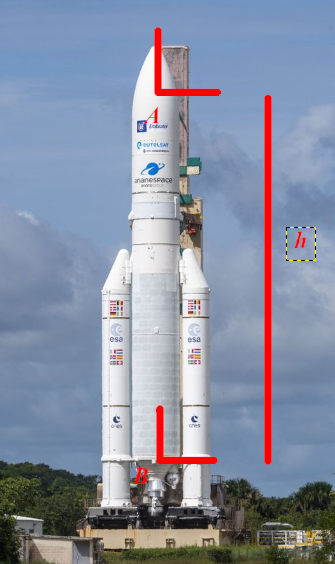
\includegraphics[width=0.4\textwidth]{img/Cohete.png} %height=4cm
	\caption{Sistema usado}
	\label{fig:cohete}
	\end{figure}
	
\begin{eqnarray}
z_{a}(0)-z_{t_{1}}=ct_{1} \\
h-\frac{1}{2}gt_{1}^{2}=ct_{1}
\end{eqnarray}

Si despues de un tiempo $t=\triangle\tau_{A} $ y B lo recibe en un tiempo 
$ t=t_{1}+\triangle\tau_{B} $ quedando como sigue%y este foton recorre una distancia dado por

%\begin{eqnarray}
%z_{A}(\triangle\tau_{A})-z_{B}(t_{1}+\triangle\tau_{B})=c(t_{1}+\triangle\tau_{B}-%\triangle\tau_{A}) \\
%\frac{g\triangle\tau_{A}^{2}}{2}+h-\frac{g(t_{1}+\triangle\tau_{B})^{2}}{2}=c(t_{1}+\triangle\tau_{B}-\triangle\tau_{A}) \\
%\frac{g\triangle\tau_{A}^{2}}{2}+h-\frac{g(t_{1}^{2}+\triangle\tau_{B}^{2}+2t_{1}\triangle\tau_{B})}{2}=c(t_{1}+\triangle\tau_{B}-\triangle\tau_{A}) \\
%\frac{g\triangle\tau_{A}^{2}}{2}+h-\frac{gt_{1}^2}{2}-\frac{g\triangle\tau_{B}^{2}}{2}-gt_{1}\triangle\tau_{B}=c(t_{1}+\triangle\tau_{B}-\triangle\tau_{A})\\
%h-\frac{gt_{1}^{2}}{2}-gt_{1}\triangle\tau_{B}+\frac{g(\triangle\tau_{A}^{2}-\triangle\tau_{B}^{2})}{2}=c(t_{1}+\triangle\tau_{B}-\triangle\tau_{A})\\
%h-\frac{gt_{1}^{2}}{2}-gt_{1}\triangle\tau_{B}=c(t_{1}+\triangle\tau_{B}-\triangle\tau_{A})
%\end{eqnarray}

%Donde en la ecuacion (7) se asume $\triangle\tau_{A}^{2}-\triangle\tau_{B}^{2}$ despreciable. Restando las ecuaciones (8) y (2) dando

\begin{equation}
-gt_{1}\tau_{B}\approx e(\triangle\tau_{B}-\triangle\tau_{A})
\end{equation}
Reemplazando $t_{1}\approx h/c$ se obtiene
\begin{equation}
\triangle\tau_{B}\approx\triangle\tau_{A}\left(\frac{1}{1-\frac{gh}{c^{2}}}\right)\approx\triangle\tau_{A}\left(1-\frac{gh}{c^{2}}\right)
\end{equation}
Esta ecuacion nos indica que el observador B veria al observador A mas rapido y viceversa, A observara a B mas lento.\\
Debido a la simetria de arriba y abajo (izquierda y derecha) esta ecuacion podria usarse para un cohete que va en "direccion izquierda a derecha", un observador en la izquierda seria como el Observador B y el observador en la derecha seria como el observador A.

	\subsection{Para un Campo debil pero no homogeneo}
A traves de la ecuacion de Scharwschild se puede tomar dos observadores con sus tiempos propios en distintos puntos del campo gravitatorio producido por el cuerpo esferico\\
Para un Observador A

\begin{equation}
d\tau_{a}^{2}=g_{\mu\upsilon}(x_{a})dx^{\mu}dx^{\upsilon}=g_{tt}(x_{a})dt^{2}
\end{equation}

\begin{equation}
d\tau_{b}^{2}=g_{\mu\upsilon}(x_{b})dx^{\mu}dx^{\upsilon}=g_{tt}(x_{b})dt^{2}
\end{equation}

Donde dividiendo estas dos ultimas ecuaciones nos daria 

\begin{equation}
d\tau_{a} =\gamma(a,b) d\tau_{b}
\end{equation}		
Donde $\gamma(a,b)$ es: \\

\begin{equation}
\gamma(a,b)=\sqrt{\frac{g_tt(a)}{g_{tt}(b)}}
\end{equation}

La ultima ecuacion es valida para metricas que sean independientes de la variable temporal (estatica) y con simetria.	\\

\clearpage %salto de pagina contando los ob. flotantes

Un ejemplo muy visual seria para dos observadores en el espacio, uno muy lejano y otro cerca del campo gravitatorio como en la figura \ref{fig:sist}.
	
	\begin{figure}[h]
	\centering
	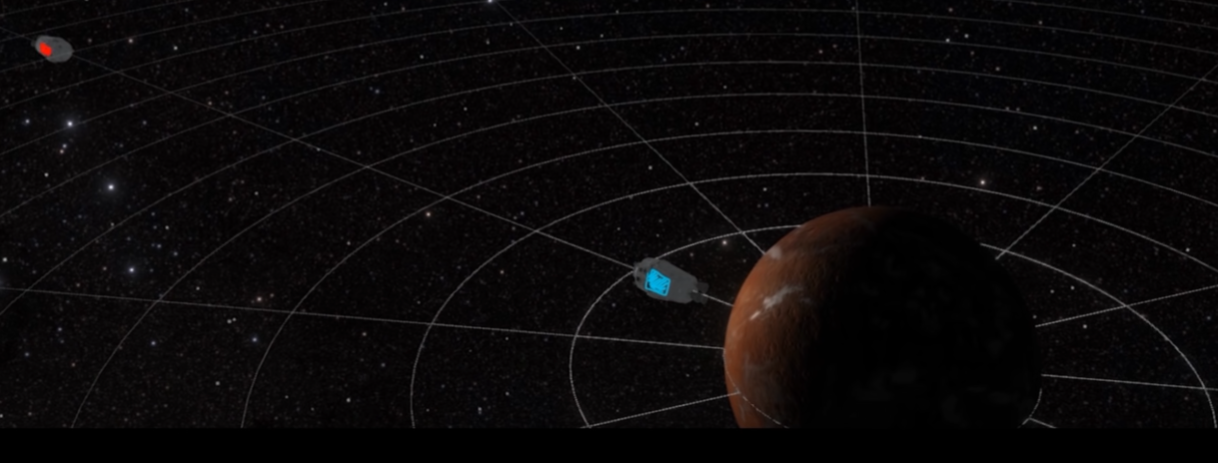
\includegraphics[width=0.5\textwidth]{img/sistema.png}
	\caption{Sistema usado de referencia. Sacado del Curso de Relatividad de Javier 		Garcia}
	\label{fig:sist}
	\end{figure}

Donde colocamos los datos del agujero negro A0620-00 se podria calcular una dilatacion casi del doble, y el observador lejano veria al observador cercano mas lento y mas 'rojo' como en la figura \ref{fig:lej}. Y en la figura \ref{fig:cerc} es el observador lejano 

	\begin{figure}[h]
	\centering
	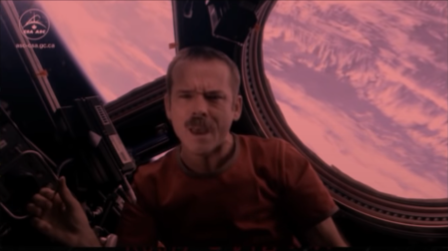
\includegraphics[width=0.5\textwidth]{img/observador lejano.png}
	\caption{Como veria el observador lejano al observador cercano}
	\label{fig:lej}
	\end{figure}

	\begin{figure}[h]
	\centering
	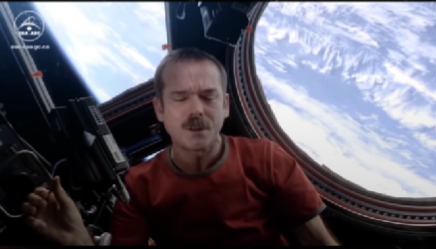
\includegraphics[width=0.5\textwidth]{img/observador cercano.png}
	\caption{Un observador lejano que cada 1s envia un pulso de luz}
	\label{fig:cerc}
	\end{figure}

\newpage

\section{Aplicaciones}
	
	\subsection{GPS}
	Una de las aplicaciones mas conocidas es en GPS, donde este necesita unas correcciones relativistas, tanto especial como general, para conseguir la sincronizacion de los relojes en cada punto de la tierra y los satelites, se realizara solo el calculo para la parte de relatividad general. Para realizar esto se realiza con respecto a la hora UTC (un reloj lejos de todo campo gravitatorio), El sistema funciona como en la figura \ref{fig:gps}
(Referir al articulo GPS2)
	
	\begin{figure}[h]
	\centering
	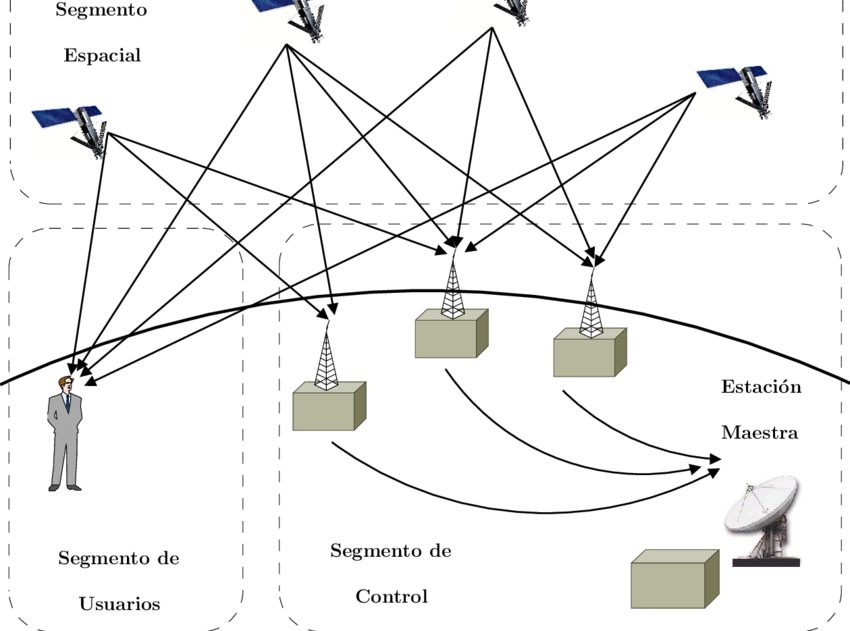
\includegraphics[width=0.5\textwidth]{img/GPS.png}
	\label{fig:gps}
	\end{figure}
	
Para los calculos usamos la formula calculada anteriormente en el caso de un campo inhomogeneo debil

\begin{equation}
T_{0}=T_{s}\sqrt{\frac{1+2\Phi_{0}}{1+2\Phi_{s}}}\to
\frac{T_{0}}{T_{s}}=1+5.278938007 x 10^{-10}
\end{equation}

Por lo que en un dia (86400 s) se acumularia en $4.561002438x10^{-5}$ segundos que representaria un error de aproximadamente $13.683 Km$

%	\subsection{Astrobiologia}
%	Nosotros no observaremos el mismo comportamiento aqui que en  el espacio(visto desde Tierra) Se observo que el tiempo corre de forma diferente ante un campo gravitatorio, pero estos no saben que esto sucede, por lo que esto afectaria a su mecanismo de reproduccion
	\section{Conclusiones}
A pesar que el efecto parezca despreciable en primera instancia, el efecto acumulativo de este podria llevar a errores apreciables.\\
Este efecto seria mas notorio mientras menor sea la diferencia entre R>2M.\\

Se observa que el tiempo propio de un observador en un mayor potencial correra mas lento que el tiempo propio que un observador lejos de este potencial.\\
Por ejemplo en la tierra(b) y el espacio(a), $\gamma(a,b)>1$, que al inicio puede ser despreciable pero por acumulacion (de misma forma que el caso del GPS) se veria un efecto apreciable
Se puede observar que el comportamiento definido por el tiempo propio de un sistema sera distinto en distintos lugares del potencial.
	\nocite{*}
	\bibliographystyle{apa}
	\bibliography{biblio}
	

\end{document}
